\documentclass[../main.tex]{subfiles}
% DOCUMENT

% \makeatletter
% \def\env@cases{%
%   \let\@ifnextchar\new@ifnextchar
%   \left\lbrace
%   \def\arraystretch{1}%
%   \array{@{}l@{\quad}l@{}}}
% \makeatother

\begin{document}
\chapter{Các thử nghiệm}\label{cuxe1c-thux1eed-nghiux1ec7m}

Để tiến hành đánh giá hiệu năng thuật toán của các chương trước, tôi sử
dụng dữ liệu được sinh ngẫu nhiên để chạy. Thuật toán được cài đặt và
chạy bằng ngôn ngữ C++17, trên máy tính để bản với hệ điều hành Fedora
39, CPU Intel i7-8700 (12) @ 4.600GHz và 128GB RAM. Việc chạy được thực hiện
với các flag tối ưu hoá \texttt{-O2} và thư viện Boost 1.73.0



\section{Tập dữ liệu}\label{tux1eadp-dux1eef-liux1ec7u}

Dữ liệu được chuẩn bị cho việc chạy các thuật toán. Có 4 kiểu dữ liệu
tương ứng với 4 kiểu mạng \(D=(N,A)\) và tập các đỉnh
\(N =\{1,2,\dots, n\}\);

\begin{itemize}
\tightlist
\item
  \textbf{Kiểu 1:} \(A = \{(i, j) \in N \times N | i < j \}\);
\item
  \textbf{Kiểu 2:}
  \(A = \{(i, i+1) | i = 1, \dots, n-1\} \cup \{(i, j) \in N \times N | i < j + 1 \text{ và } U_{i, j} < 0.5\}\)
  với mỗi \((i, j)\), giá trị \(U_{i, j}\) được lấy độc lập từ phân phối
  chuẩn \([0, 1]\) hay \(U_{i, j} \sim U[0,1]\)
\item
  \textbf{Kiểu 3:} \(A = \{(i, j) \in N \times N | i < j < i + 4 \}\);
\item
  \textbf{Kiểu 4:}
  \(A = \{(i, j+1) | i = 1, \dots, n-1\} \cup \{(i, j) \in N \times N | i < j +1 \text{ và } U_{i, j} < 1/ |j-i|\}\)
  với \(U_{i, j} \sim U[0,1]\) cho mỗi \((i, j)\).
\end{itemize}

\subsection{Tóm tắt cho mỗi kiểu mạng}\label{tom-tat-moi-kieu-mang}

\textbf{Kiểu 1:}

\begin{itemize}
\tightlist
\item
  Mỗi cặp đỉnh bất kì đều được nối với nhau bằng một cung.
\item
  Mật độ của mạng: \(0.5\) (mỗi đỉnh kết nối đến tất cả các đỉnh khác).
\end{itemize}

\textbf{Kiểu 2:}

\begin{itemize}
\tightlist
\item
  Bao gồm nửa số cung có trong Kiểu 1,
\item
  Để đảm bảo luôn có ít nhất một đường đi khả thi, mọi cung giữa các
  đỉnh liên tiếp vẫn được giữ lại.
\item
  Mật độ mạng: khoảng \(0.25\).
\end{itemize}

\textbf{Kiểu 3:}

\begin{itemize}
\tightlist
\item
  Mỗi đỉnh được nối với ba đỉnh tiếp theo theo số thứ tự.

  \begin{itemize}
  \tightlist
  \item
    Ví dụ: đỉnh $1$ sẽ nối với đỉnh $2$, $3$ và $4$.
  \end{itemize}
\item
  Mật độ mạng: khoảng \(3/n\).
\end{itemize}

\textbf{Kiểu 4:}

\begin{itemize}
\tightlist
\item
  Khả năng tồn tại một cung giữa hai đỉnh phụ thuộc vào khoảng cách giữa
  chúng.
\item
  Càng xa nhau về mặt số thứ tự thì càng giảm khả năng xuất hiện cung.
\item
  Để đảm bảo luôn có ít nhất một đường đi khả thi, tất cả các cung giữa
  các đỉnh liên tiếp vẫn được giữ lại.
\item
  Mật độ mạng: khoảng \(\log n!/(n^2)\).
\end{itemize}

\section{Hàm thời gian}\label{huxe0m-thux1eddi-gian}

Để đánh giá mức độ ảnh hưởng của hàm thời gian di chuyển đến hiệu năng
của thuật toán, có ba loại hàm được sử dụng. \autoref{fig:11} minh hoạ cho mỗi
loại. Hàm thời gian di chuyển được tạo ra như sau: với mỗi cung
\((i,j)\), sử dụng nội suy tuyến tính từng khúc của một hàm \(f\) (mô tả
chi tiết ở dưới) với các điểm là số nguyên.

\textbf{Loại 1:} \(f\) là đa thức bậc $4$:

\begin{multline}
   f\big([0, \frac{T}{4}, \frac{T}{2}, \frac{3T}{4}, T]\big) \\
   =
   \begin{cases} 
    [1.6, 1, 1.05, 1, 1.6](B_{i,j} \frac{|j − i|}{10}), & \text {nếu } U_{i,j} < \frac{1}{3}, \\ 
    [2, 1, 1.5, 1, 2](B_{i,j} \frac{|j − i|}{10}), & \text {nếu } \frac{1}{3} \leq U_{i,j} < \frac{2}{3}, \\ 
    [2.5, 1, 1.75, 1, 2.5](B_{i,j} \frac{|j − i|}{10}), & \text{ còn lại},
    \end{cases}
    \end{multline}
    Với \(B_{i, j}, U_{i, j} \sim U[0, 1]\).

\textbf{Loại 2:} \(f\) là đa thức bậc $6$:
\begin{multline}
    f\big([0, \frac{T}{6}, \frac{T}{3}, \frac{T}{2}, \frac{2T}{3}, \frac{5T}{6}, T]\big) \\
    = 
    \begin{cases} 
    [1, 1.6, 1, 1.05, 1, 1.6, 1](B_{i,j} \frac{|j − i|}{10}), & \text {nếu }  U_{i,j} < \frac{1}{3}, \\ 
    [1, 2, 1, 1.5, 1, 2, 1](B_{i,j} \frac{|j − i|}{10}), & \text {nếu } \frac{1}{3} \leq U_{i,j} < \frac{2}{3}, \\ 
    [1, 2.5, 1, 1.75, 1, 2.5, 1](B_{i,j} \frac{|j − i|}{10}), & \text{ còn lại},
    \end{cases}
\end{multline}

Với \(B_{i, j}, U_{i, j} \sim U[0, 1]\).

\textbf{Loại 3:} 
\(f(t) = (j − i) + sin (B_{i,j} \times t), \text{ với } B_{i,j} \sim U[0, 1].\)

% \begin{figure}
% \centering
% 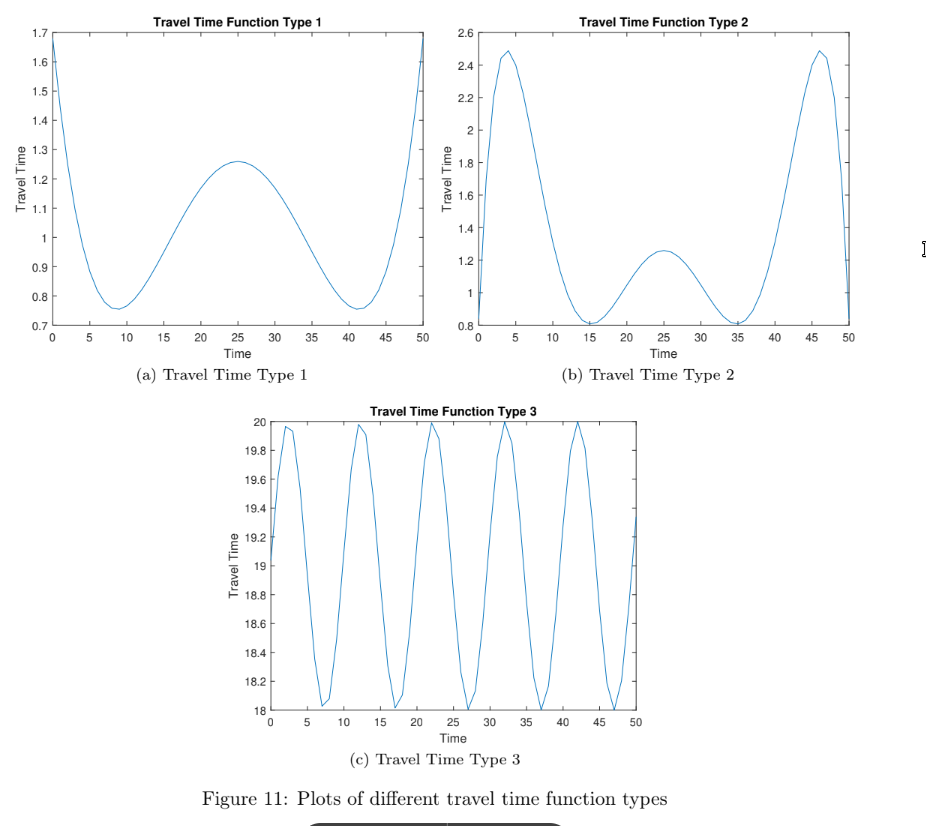
\includegraphics{images/Figure11.png}
% \caption{Figure 11}
% \label{fig:11}
% \end{figure}

\begin{figure}
  \centering

  \subcaptionbox{Loại 1\label{fig:11a}}{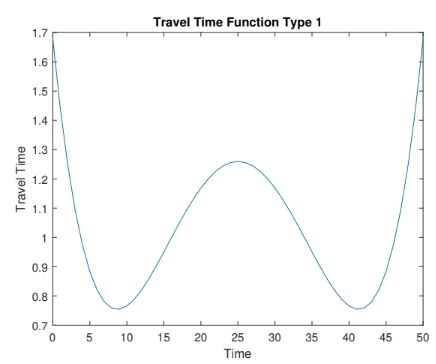
\includegraphics[width=.45\textwidth]{edited-images/Figure11a.jpg}}
  \subcaptionbox{Loại 2\label{fig:11b}}{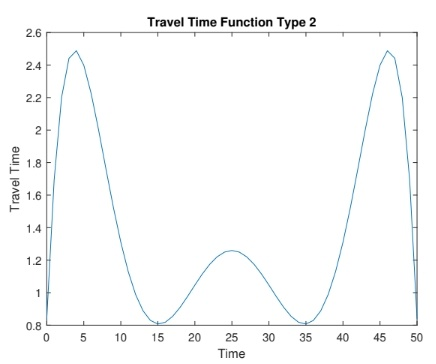
\includegraphics[width=.45\textwidth]{edited-images/Figure11b.jpg}}\\

  \subcaptionbox{Loại 3\label{fig:11c}}{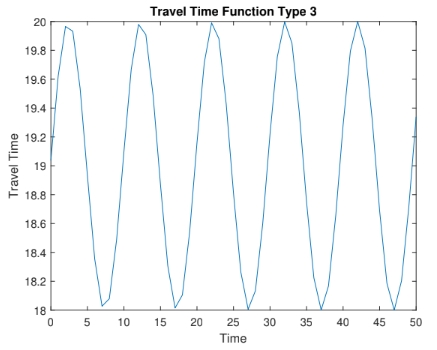
\includegraphics[width=.45\textwidth]{edited-images/Figure11c.jpg}}

  \caption{Biểu diễn ba loại hàm thời gian di chuyển}
  \label{fig:11}
\end{figure}

\subsection{Nguồn gốc của các hàm thời
gian}\label{nguux1ed3n-gux1ed1c-cux1ee7a-cuxe1c-huxe0m-thux1eddi-gian}

Hàm \textbf{Loại 1} được lấy ý tưởng từ \cite{figliozzi2012time} về
việc chia 5 khoảng thời gian bằng nhau, mỗi khoảng có tốc độ di chuyển
không đổi. Tốc độ di chuyển cơ sở (lấy ngẫu nhiên) được nhân với các hệ
số lần lượt là \(1.6, 1.0, 1.05, 1.0\) và \(1.6\) tại các thời điểm
\(0, \frac 1 4 T, \frac 1 2 T, \frac 3 4 T\) và \(T\) tương ứng. Sau đó sử dụng nội suy đa
thức qua các điểm này để tạo nên hàm liên tục. Cuối cùng chuyển chúng về
dạng hàm tuyến tính từng khúc bằng cách nội suy tuyến tính từng khúc của
đa thức trên tại các điểm nguyên.

Hàm \textbf{Loại 2} được mở rộng từ \textbf{Loại 1} bằng cách thêm hai
điểm ở đầu và cuối để tăng độ khó (tăng bậc).

Hàm \textbf{Loại 3} gây ra nhiều thách thức cho thuật toán vì chúng
không đồng pha trên các cung có nhiều điểm cực tiểu và cực đại cục bộ.

Ngoài ra các hàm khác được đề xuất trong \cite{figliozzi2012time} cũng
được thử nghiệm, nhưng thuật toán này tìm ra nghiệm chỉ sau vài lần lặp.
Các nghiệm tối ưu thường bắt đầu ở thời điểm sớm nhất hoặc muộn nhất có
thể, do đó không giúp ích cho việc phân tích hiệu năng của thuật toán.

Hiệu năng của cả hai bài toán với phương pháp DDD phụ thuộc rất nhiều
vào việc tính toán UTT: có thể tính toán một cách hiệu quả thời gian tối
thiểu di chuyển qua các cung ngay khi bắt đầu chạy thuật toán. Bảng tra
cứu là một cấu trúc dữ liệu hiệu quả cho việc tính toán trước khi chạy.

\section{Kịch bản và cài
đặt}\label{kux1ecbch-bux1ea3n-vuxe0-cuxe0i-ux111ux1eb7t}

Phần này sẽ bàn về ảnh hưởng của việc chọn điểm dừng đến hiệu năng của
thuật toán.

Với bài toán MDP, giả sử cận dưới đang là \(LB^t\) và \(t^+\) là thời
gian đến đỉnh \(n\) của ABSPT ngay sau \(\overline{\mathcal{B}}^t\). Kí
hiệu cho nút trong \(\overline{\mathcal{B}}^t\) là \((i,t_i)\) và trong
\(\overline{\mathcal{B}}^{t^+}\) là \((i, t_i^+)\). Chọn cung \((i,j)\)
sao cho mỗi cung thuộc \(\overline{\mathcal{B}}^{t}\) có điểm dừng trong
khoảng thời gian \((t_i, t_i^+)\) và có chỉ số nhỏ nhất (khi xét các
đỉnh từ \(1\) đến \(n\)). Dưới đây là ba cách chọn điểm gãy cho
\(c_{i,j}(t)\) với \(t\in (t_i, t_i^+)\):

\begin{enumerate}
\def\labelenumi{\arabic{enumi}.}
\tightlist
\item
  Chọn một điểm bất kì (\(RAND\))
\item
  Chọn điểm trung vị (trong tập các điểm dừng sắp xếp theo thời gian)
  (\(MED\))
\item
  Chọn điểm có giá trị \(c_{i, j}(t)\) nhỏ nhất với
  \(t\in (t_i, t_i^+)\) (\(MIN\)).
\end{enumerate}

Với bài toán MTTP, ta so sánh hai kịch bản chọn điểm dừng để thêm vào
danh sách \(L^i\) ở mỗi lần lặp như sau:

\begin{itemize}
\tightlist
\item
  \textbf{Thêm một điểm dừng (S):} Thêm một điểm dừng cho một trong các
  đường con ở mỗi lần lặp.
\item
  \textbf{Thêm nhiều điểm dừng (M):} Thêm một điểm dừng cho mọi đường
  con ở mỗi lần lặp.
\end{itemize}

Quy tắc chọn điểm dừng như sau: Để chọn điểm cần thêm vào, ta xác định
một chuỗi các \(mangrove\) hoàn chỉnh được sử dụng bởi đường đi UTT kí
hiệu \(P_{LB}\). Mỗi \(mangrove\) hoàn chỉnh được tạo ra từ một BP, giả
sử đó là điểm \((i,t)\). Khi đó, nếu \((i,t^+)\) là điểm ngay sau
\((i,t)\) trong \(L^i\) và có một BP chưa được giải quyết tại đỉnh \(i\)
có thời gian giữa \(t\) và \(t^+\), thì điểm \((i,t^+)\) này sẽ xem xét
để chọn. Tập hợp các điểm như vậy gọi là tập ứng viên. Cách chọn điểm từ
tập ứng viên thuộc một trong ba cách ở trên (\(RAND, MED, MIN\)). Với
kịch bản \textbf{(S)}, thêm một BP của đỉnh \(i\) cho \(i-mangrove\)
hoàn chỉnh đầu tiên được dùng bởi đường đi UTT từ \(1\) đến \(n\), nếu
BP ứng viên tồn tại. Trong kịch bản \textbf{(M)}, thêm một BP vào mỗi
\(mangrove\) hoàn chỉnh được dùng bởi đường đi UTT, nếu BP ứng viên
tương ứng tồn tại.

\textbf{Đánh giá hiệu năng của việc lựa chọn BP:}

Đầu tiên, với bài toán MDP, kết quả được biểu diễn ở \autoref{fig:12} bằng biểu
đồ hộp với các tỉ số: thời gian chạy, số lần lặp và số BP được giải
quyết cho cách chọn \(RAND\) và \(MIN\) khi so sánh với \(MED\).

% \begin{figure}
% \centering
% 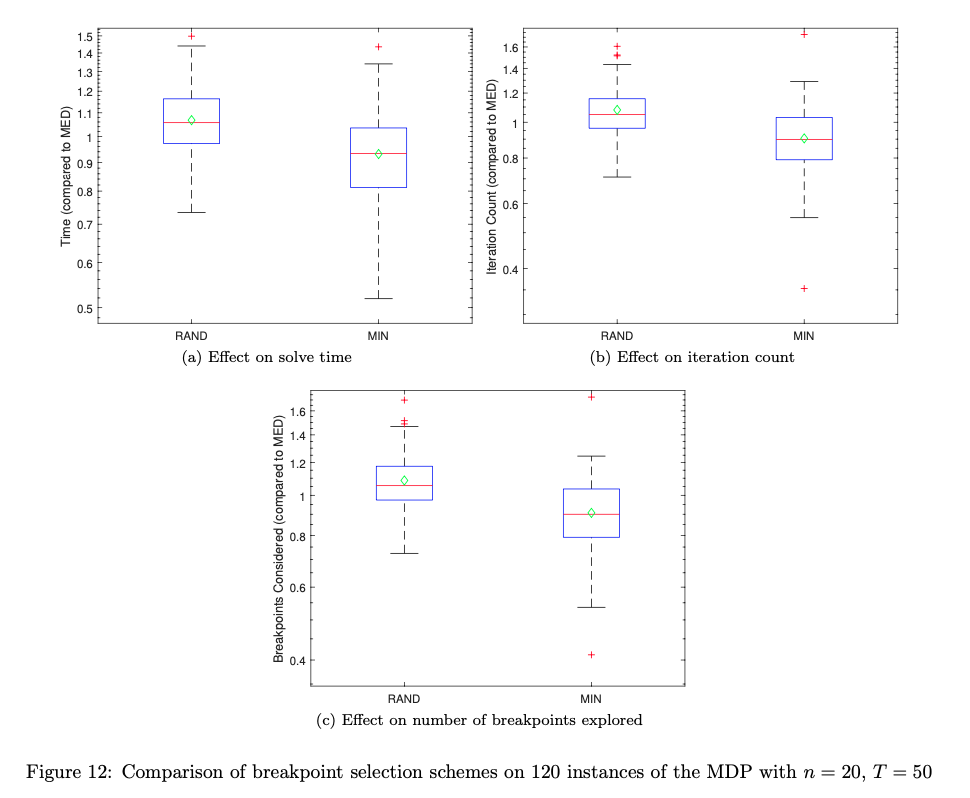
\includegraphics{images/Figure12.png}
% \caption{So sánh các cách chọn với 120 mẫu của bài toán MDP cho \(n=20, T=50\)}
% \label{fig:12}
% \end{figure}

\begin{figure}
  \centering
  \subcaptionbox{Thời gian chạy\label{fig:12a}}{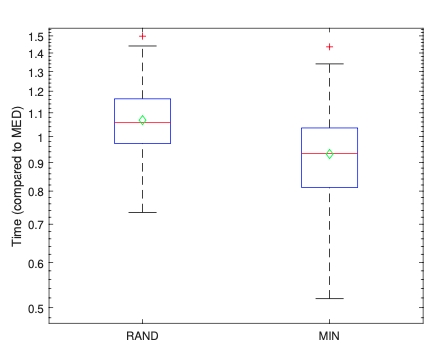
\includegraphics[width=.45\textwidth]{edited-images/Figure12a.jpg}}
  \subcaptionbox{Số lần lặp\label{fig:12b}}{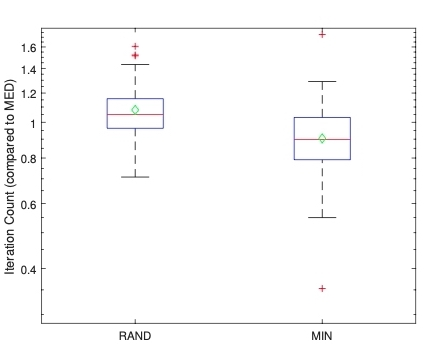
\includegraphics[width=.45\textwidth]{edited-images/Figure12b.jpg}}\\

  \subcaptionbox{Số BP được giải quyết\label{fig:12c}}{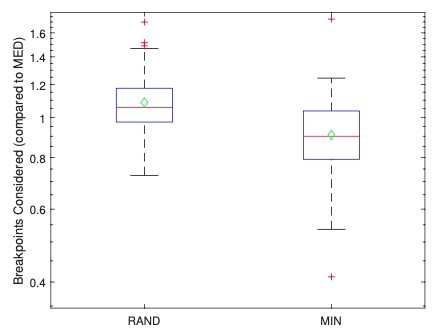
\includegraphics[width=.45\textwidth]{edited-images/Figure12c.jpg}}
  \caption{So sánh các cách chọn với 120 mẫu của bài toán MDP cho \(n=20, T=50\)}
  \label{fig:12}
\end{figure}

\begin{itemize}
\tightlist
\item
  \textbf{Biểu đồ hộp:}

  \begin{itemize}
  \tightlist
  \item
    Hình thoi màu xanh lá cây biểu thị giá trị trung bình.
  \item
    Đường ngang màu đỏ biểu thị giá trị trung vị.
  \end{itemize}
\item
  \textbf{Trục Y:}~thang đo logarit.
\end{itemize}

Qua quan sát, cách chọn \(MIN\) cho kết quả tốt nhất trong cả ba tiêu
chí hiệu năng (thời gian chạy, số lần lặp và số BP được giải quyết). Do
đó, \(MIN\) là lựa chọn ưu tiên trong ba cách.

Tiếp theo, ta đánh giá tác động của cách chọn BP và số BP được xử lý
trong mỗi lần lặp khi giải bài toán MTTP.

% \begin{figure}
% \centering
% 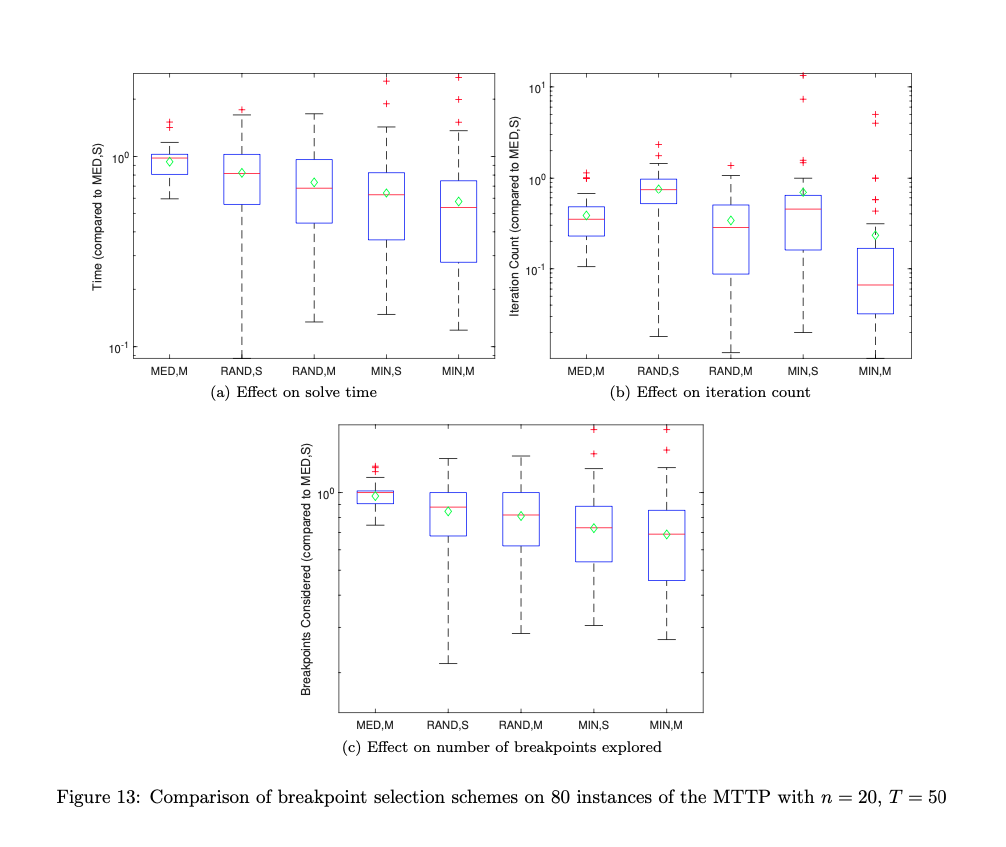
\includegraphics{images/Figure13.png}
% \caption{So sách các cách chọn với 80 mẫu của bài toán MTTP cho
% \(n=20, T=50\)}
% \label{fig:13}
% \end{figure}

\begin{figure}
  % \begin{subfigure}{.5\linewidth}
  %   % \centering
  %   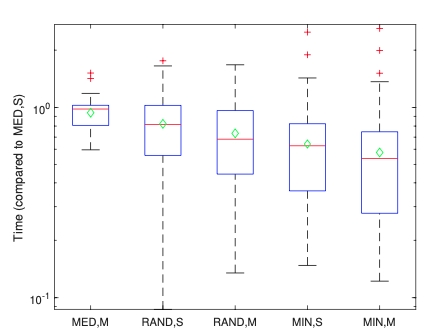
\includegraphics{edited-images/Figure13a.jpg}
  %   \caption{Thời gian chạy}
  %   \label{fig:13a}
  % \end{subfigure}
  % \hfill
  % \begin{subfigure}{.5\linewidth}
  %   % \centering
  %   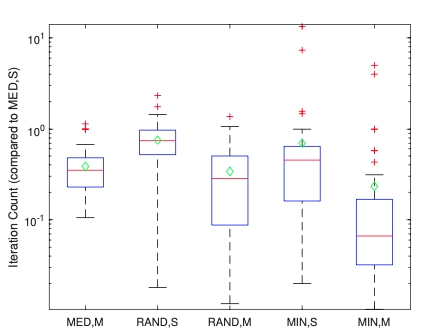
\includegraphics{edited-images/Figure13b.jpg}
  %   \caption{Số lần lặp}
  %   \label{fig:13b}
  % \end{subfigure}\\[1ex]
  % \begin{subfigure}{\linewidth}
  %   \centering
  %   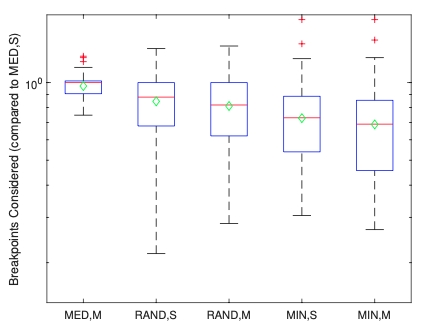
\includegraphics{edited-images/Figure13c.jpg}
  %   \caption{Số BP được giải quyết}
  %   \label{fig:13c}
  % \end{subfigure}

  \centering
  \subcaptionbox{Thời gian chạy\label{fig:13a}}{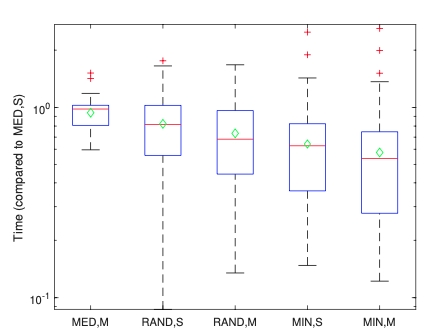
\includegraphics[width=.45\textwidth]{edited-images/Figure13a.jpg}}
  \subcaptionbox{Số lần lặp\label{fig:13b}}{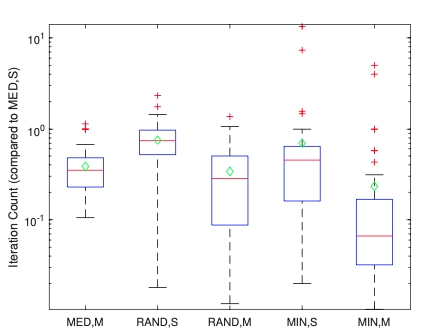
\includegraphics[width=.45\textwidth]{edited-images/Figure13b.jpg}}\\

  \subcaptionbox{Số BP được giải quyết\label{fig:13c}}{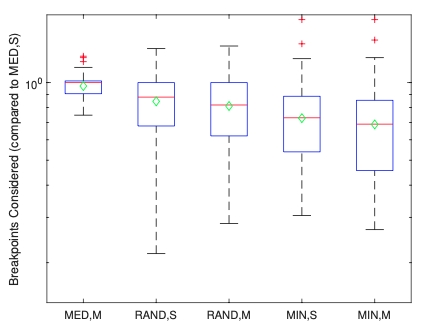
\includegraphics[width=.45\textwidth]{edited-images/Figure13c.jpg}}
  \caption{So sánh các cách chọn với 80 mẫu của bài toán MTTP cho \(n=20, T=50\)}
  \label{fig:13}
\end{figure}

\autoref{fig:13} là biểu đồ hộp của các tỷ số: thời gian chạy, số lần lặp và số
BP được giải quyết cho các kịch bản: (\(RAND\), \textbf{S}), (\(RAND\),
\textbf{M}), (\(MED\), \textbf{M}), (\(MIN\), \textbf{S}), (\(MIN\),
\textbf{M}) khi so sánh với kịch bản (\(MED\), \textbf{S}). Chỉ các mẫu
với hai hàm thời gian di chuyển được sử dụng vì thời gian chạy với hàm
thứ ba trở đi là rất lớn (sẽ đề cập chi tiết sau). Qua quan sát, kịch
bản (\(MIN\), \textbf{M}) là lựa chọn tốt nhất (theo cả ba tiêu chí).
Thêm vào đó, việc giải quyết một BP cho các đường con trong một lần lặp
mang lại lợi ích đáng kể. Khá bất ngờ khi kịch bản (\(RAND\),
\textbf{S}) lại vượt trội cả (\(MED\), \textbf{S}) và (\(MED\),
\textbf{M}) về thời gian chạy trung bình.

\section{Những lợi ích của
DDD}\label{nhux1eefng-lux1ee3i-uxedch-cux1ee7a-ddd}

Trong phần này tôi sẽ so sánh hiệu năng của thuật toán DDD với các thuật
toán liệt kê BP, với kịch bản chọn là \(MIN\). Trong bài toán MTTP sử
dụng việc khám phá nhiều BP cho mỗi lần lặp.

\autoref{table:mdp1} trình bày kết quả chạy trung bình với 10 mẫu được sinh ngẫu
nhiên, với mạng lưới có kích thước khác nhau (\(n=20,30,50\) và
\(T=50\)) với 4 loại hàm thời gian di chuyển cho bài toán MDP.

\begin{figure}
\centering
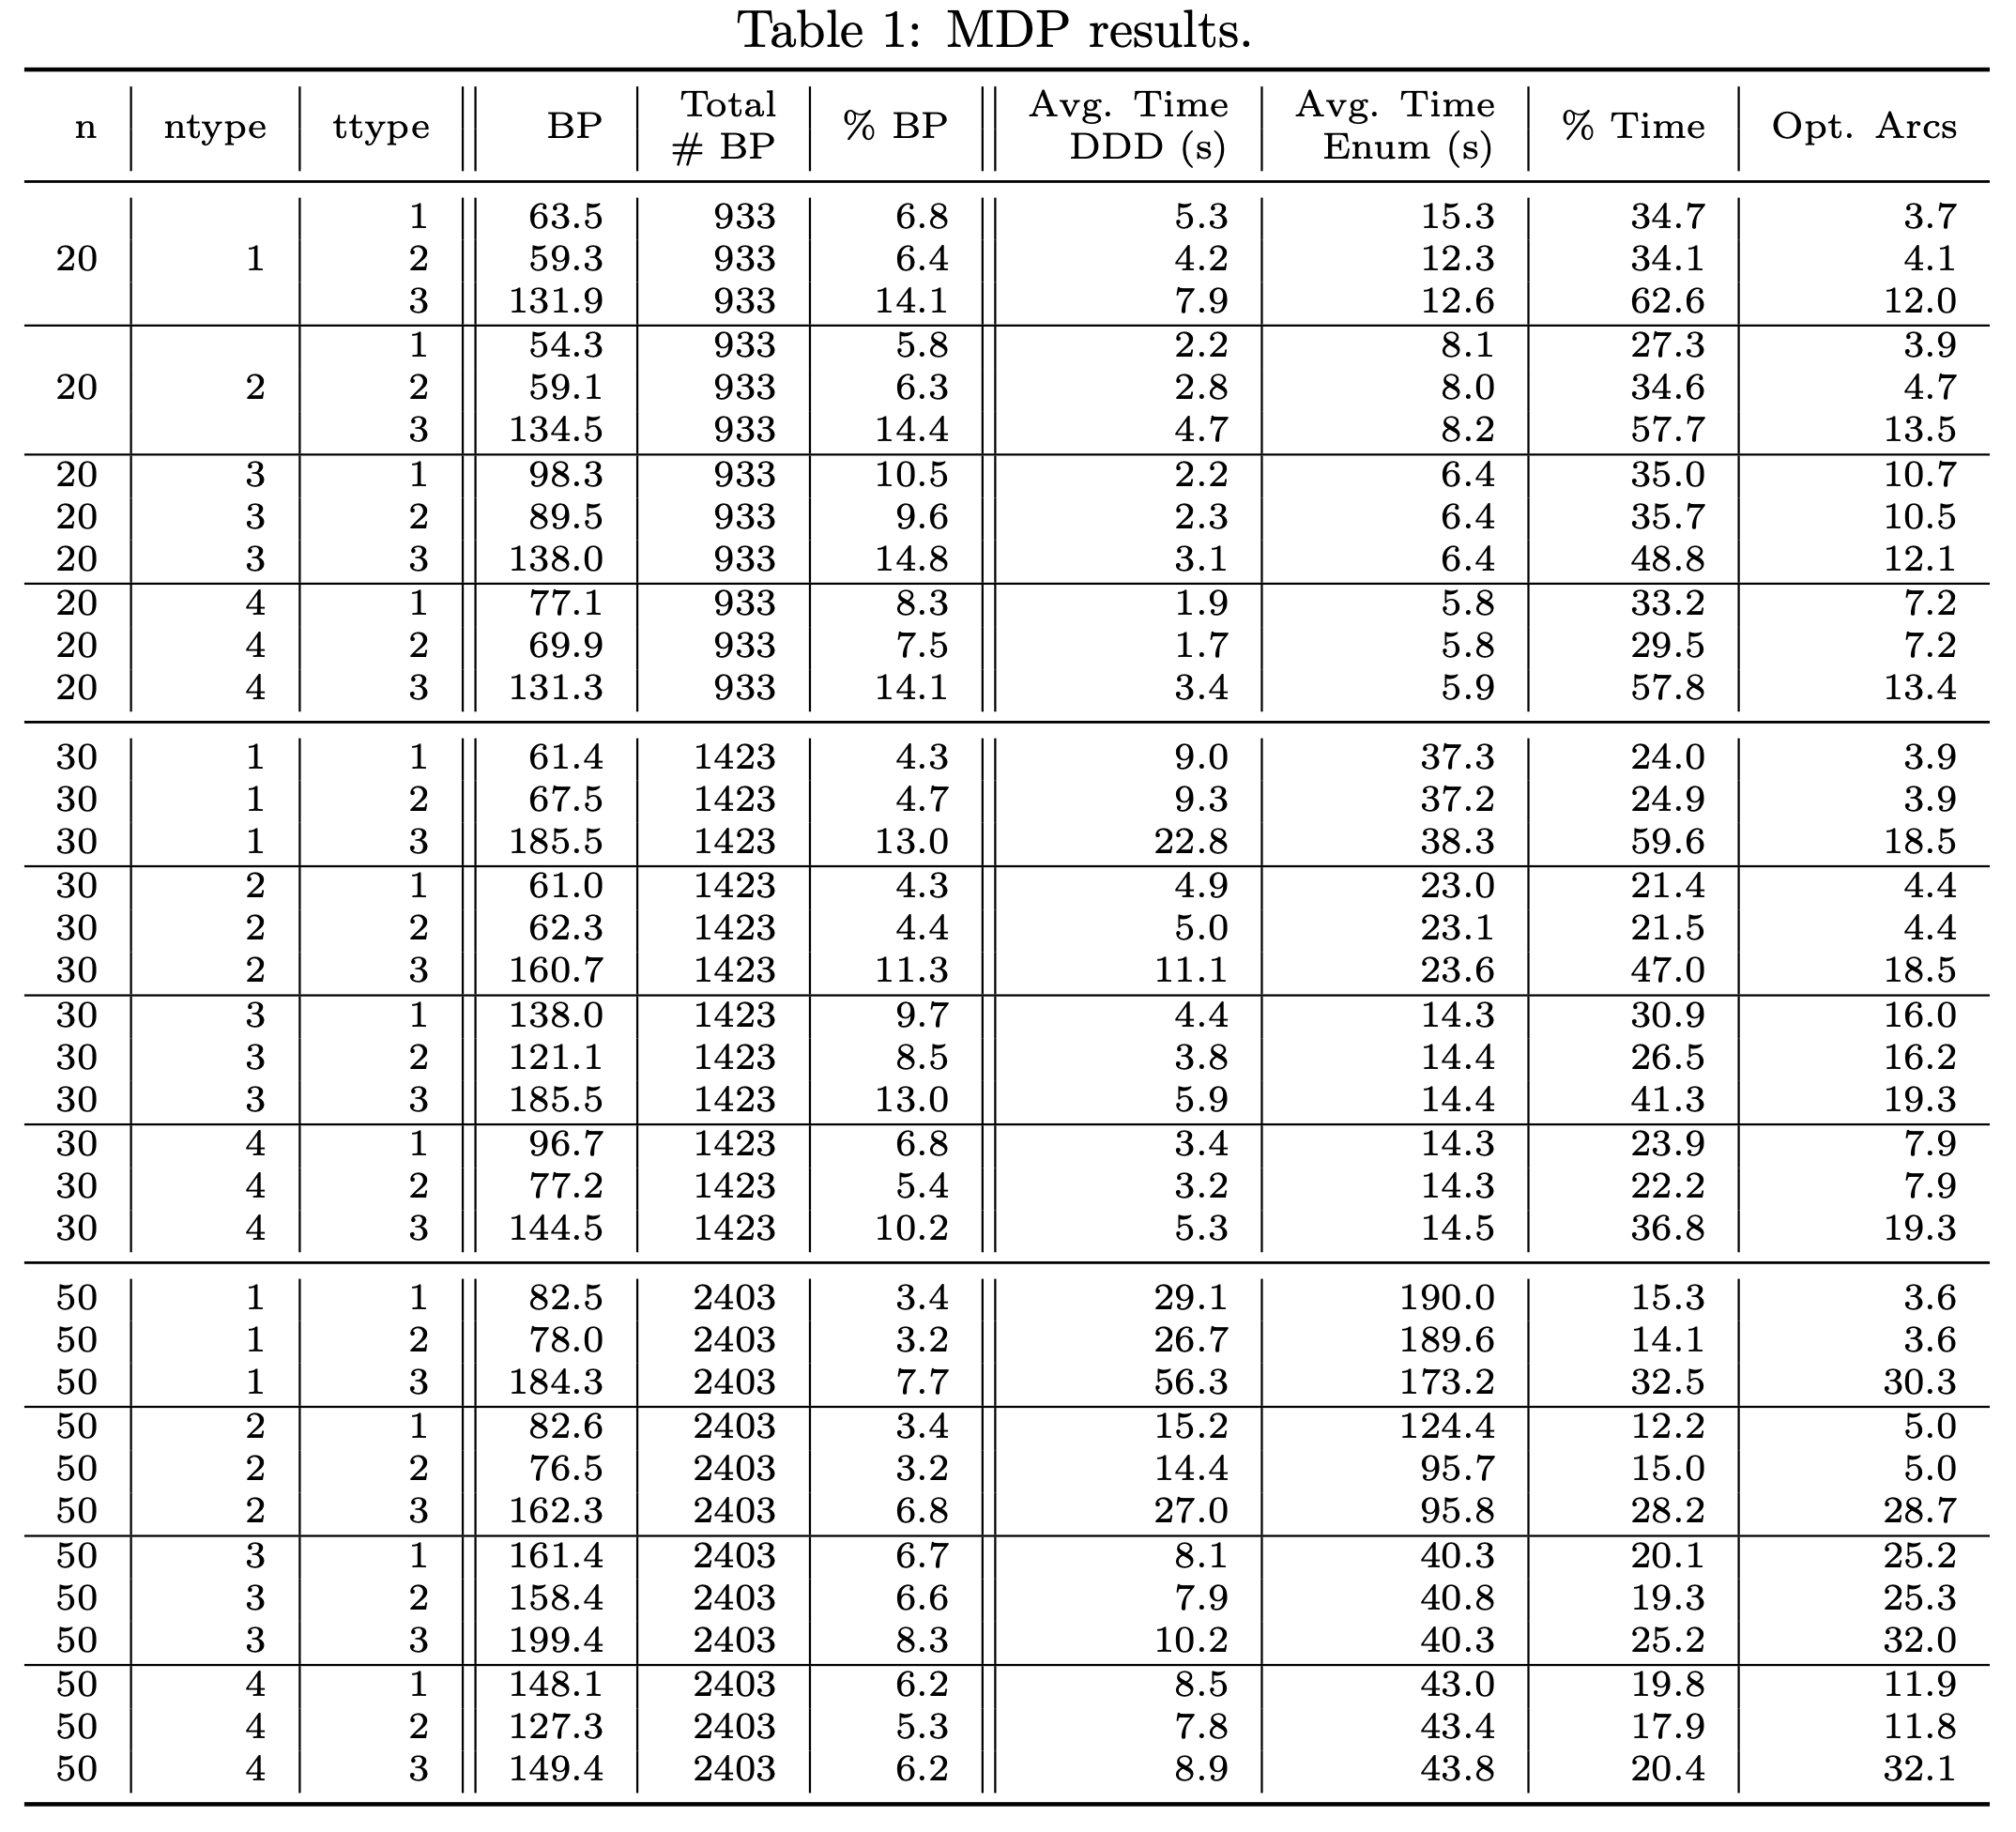
\includegraphics{images/Table1.png}
\caption{Kết quả của MDP}
\label{table:mdp1}
\end{figure}

\begin{table}[]
  \caption{Kết quả của MDP với \(n=[30, 50]\) và \(T=20\)}
  \label{table:mdp-result}
  \resizebox{\textwidth}{!}{
    \begin{tabular}{|p{0.5cm}|p{1cm}|p{1cm}||p{2cm}|p{1.5cm}|p{2cm}|p{2cm}|p{2.5cm}|p{2.5cm}|p{1.5cm}|p{1cm}|}
    % \begin{tabular}{SSS|SSSSSSS}
    % \hline
    % \Xhline{2pt}
    \toprule
    n  & g-type & t-type & Avg. BP         & Total BP & \% BP            & Avg. Arcs          & Avg. Time DDD (ms)    & Avg. Time Enum (ms) &  \% Time         & Iters \\ \midrule
    30 & 1     & 1     & 32.60           & 553      & 5.90             & 5.10               & 38.10                 & 348                    & 10.95         & 398        \\ 
    30 & 1     & 2     & 32.60           & 553      & 5.90             & 5.10               & 40.30                 & 378.90                 & 10.64         & 393        \\ 
    30 & 2     & 1     & 36.80           & 553      & 6.65             & 9                  & 22.50                 & 212.80                 & 10.57         & 470        \\ 
    30 & 2     & 2     & 38.80           & 553      & 7.02             & 9                  & 23.30                 & 231.60                 & 10.06         & 487        \\ 
    30 & 3     & 1     & 29.90           & 553      & 5.41             & 6.80               & 28.40                 & 296.40                 & 9.58          & 351        \\ 
    30 & 3     & 2     & 32.60           & 553      & 5.90             & 6.70               & 30.90                 & 321.90                 & 9.60          & 389        \\ \midrule
    50 & 1     & 1     & 36.90           & 933      & 3.95             & 7.50               & 81.40                 & 1112.70                & 7.32          & 440        \\ 
    50 & 1     & 2     & 49.20           & 933      & 5.27             & 7.50               & 109.10                & 1192.70                & 9.15          & 584        \\ 
    50 & 2     & 1     & 47.60           & 933      & 5.10             & 13                 & 52.80                 & 622.40                 & 8.48          & 590        \\ 
    50 & 2     & 2     & 46.60           & 933      & 4.99             & 13                 & 52.10                 & 686.30                 & 7.59          & 562        \\ 
    50 & 3     & 1     & 47              & 933      & 5.04             & 9                  & 88.60                 & 903.30                 & 9.81          & 589        \\ 
    50 & 3     & 2     & 41.20           & 933      & 4.42             & 8.90               & 75                    & 965.60                 & 7.77          & 478        \\ \bottomrule
  \end{tabular}
  }
\end{table}

Trong bảng có các cột với ý nghĩa như sau: Trung
bình số BP khám phá được bởi phương pháp DDD, số BP khám phá được bằng phương pháp liệt kê
(tổng số BP của mẫu), tỉ lệ phần trăm số BP được khám phá. Thêm vào đó
còn có thời gian chạy (đơn vị giây) của phương pháp DDD, thời gian chạy
của phương pháp liệt kê, tỉ lệ phần trăm thời gian chạy của DDD với
phương pháp liệt kê, và số lượng cung trung bình trong nghiệm tối ưu.
Lưu ý rằng tổng sô BP có thể có trong các mẫu này là
\(|N − 1| \times (T − 1) + 2\), khác với công thức
\(|A| \times (T − 1) + 2\) của \cite{foschini2011complexity}. Vì đối
với các cung có cùng hai đỉnh đầu cuối, ta chỉ cần xử lý một lần.

Kết quả cho thấy phương pháp DDD chỉ cần khám phá một phần nhỏ (từ
\(3.2\%\) đến \(14.8\%\)) tổng số BP. Điều này cho thấy phương pháp này
hoạt động hiệu quả, chỉ tập trung vào các BP tiềm năng thay vì toàn bộ.
Tuy nhiên như đã đề cập từ trước, hàm thời gian di chuyển loại 3 gây ra
nhiều thách thức nhất: nhiều BP cần khám phá hơn tương ứng với thời gian
chạy lâu hơn. Không ngoài dự đoán, phương pháp liệt kê ít bị tác động
bởi loại hàm thời gian di chuyển, nhưng phụ thuộc vào mật độ mạng lưới
(số nút và cung). Ta cũng có thể thấy rằng khi kích cỡ mẫu tăng lên thì
lợi ích của phương pháp DDD càng rõ rệt.

\autoref{table:mttp1} trình bày kết quả chạy trung bình với 10 mẫu được sinh ngẫu
nhiên, với mạng lưới có kích thước khác nhau (\(n=20,30\) và \(T=50\))
với 4 loại hàm thời gian di chuyển cho bài toán MTTP.

\begin{figure}
\centering
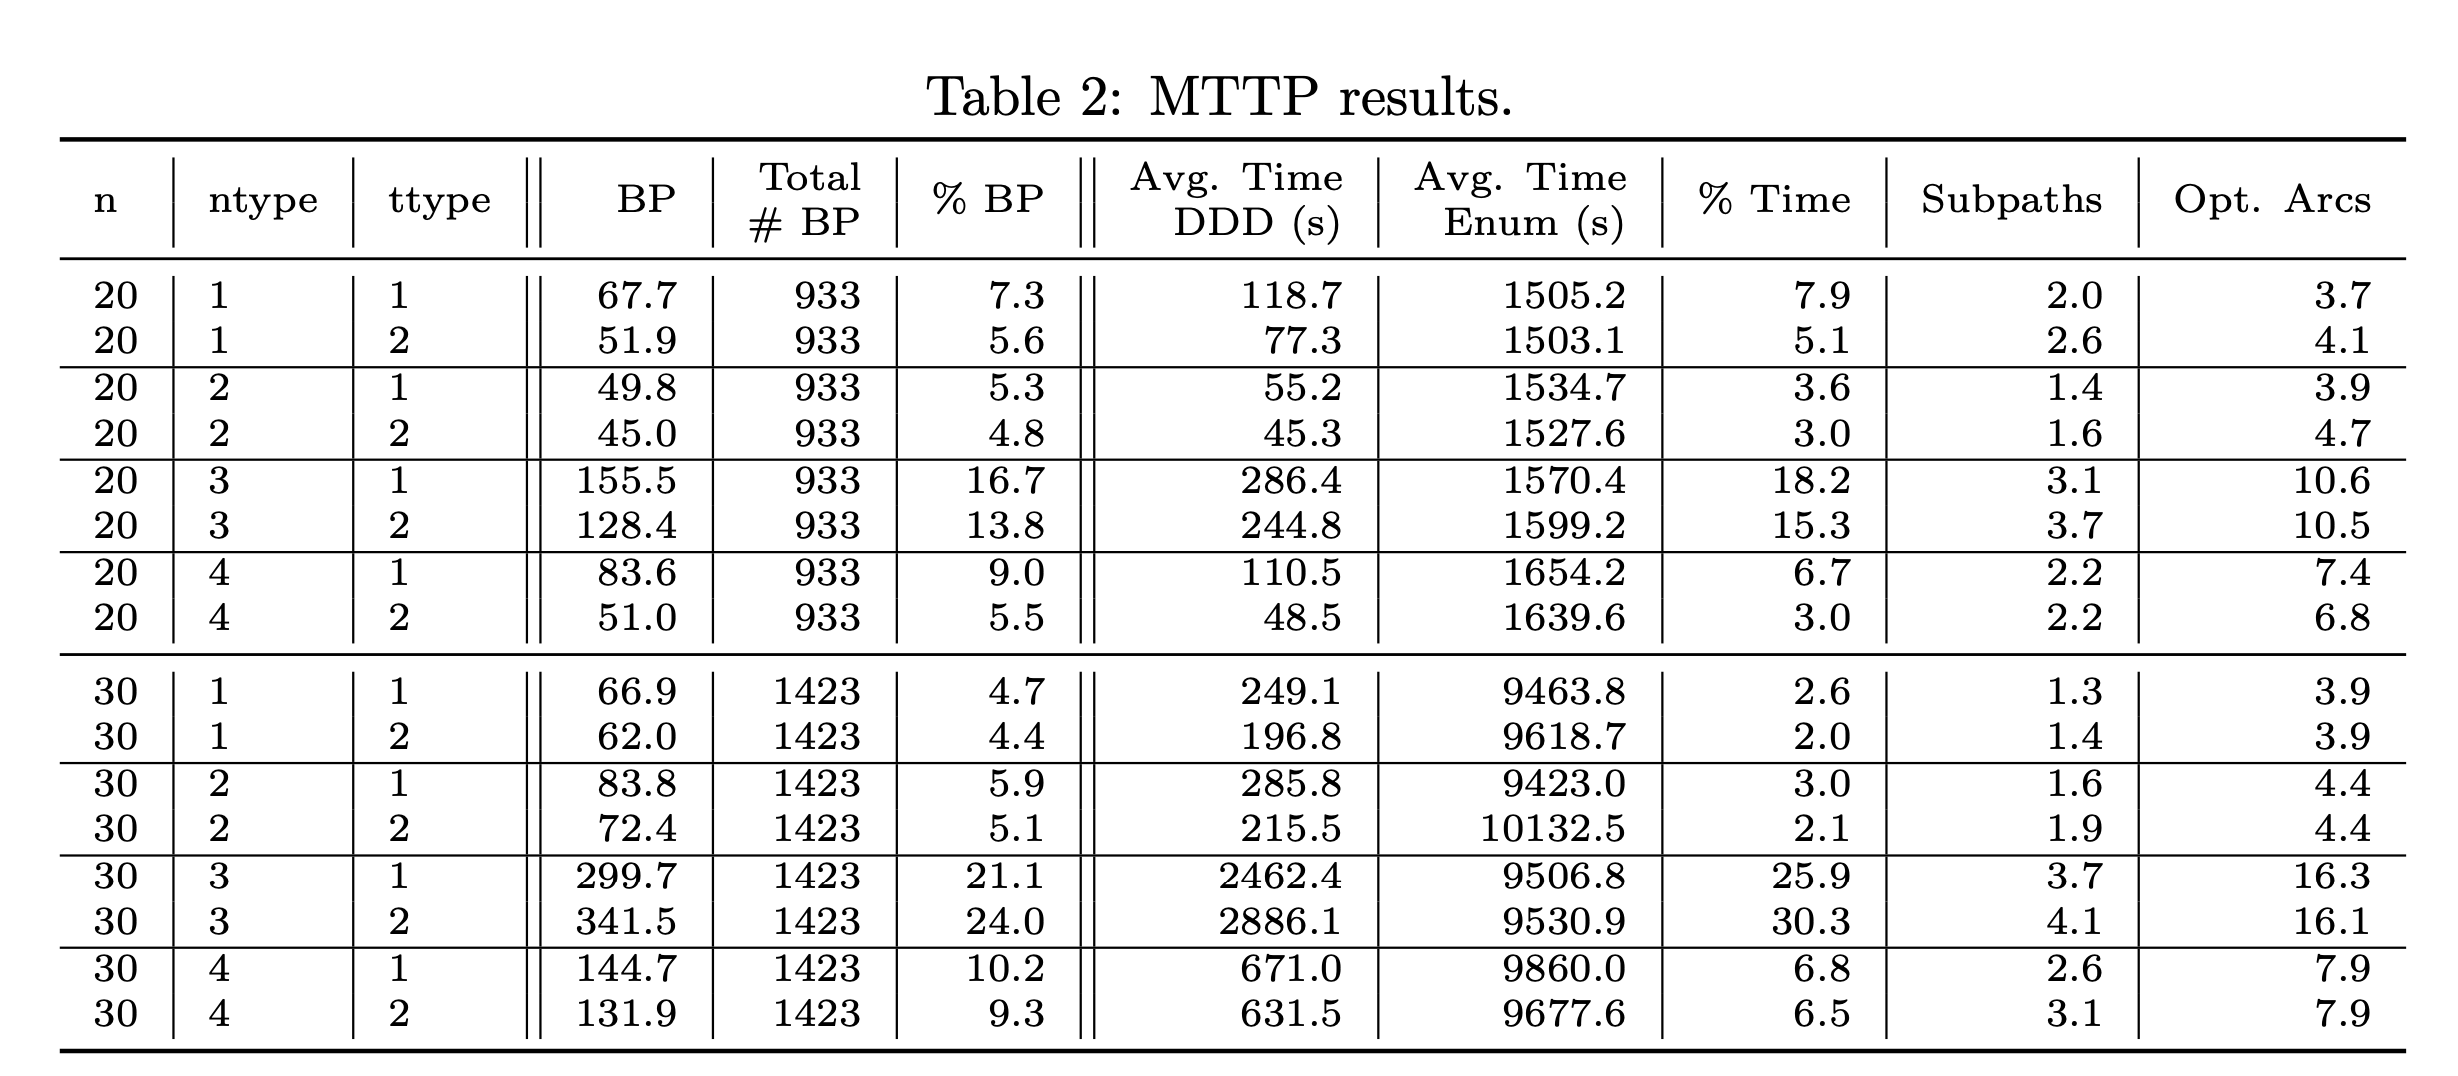
\includegraphics{images/Table2.png}
\caption{Kết quả của MTTP}
\label{table:mttp1}
\end{figure}

\begin{table}[]
  \caption{Kết quả của MTTP với \(n=[30, 50]\) và \(T=20\)}
  \label{table:mttp-small}
  % \begin{tabular}{|lllllllllllllll|}
  % reduce size of this table
  \resizebox{\textwidth}{\textwidth}{
  \begin{tabular}{|p{0.5cm}|p{1cm}|p{1cm}||*{11}{p{1.5cm}|}}
    \toprule
    n  & g-type & t-type & Avg. BP & Total BP & \% BP & Add. Time (ms) & SP. Time (ms) & Avg. Arcs & Avg. Sub-paths & Avg. DDD Time & Avg. Enum Time & \% Time & Iters \\ \midrule
    30 & 1      & 1      & 151     & 553      & 27.3  & 166.5          & 407.4         & 5.1       & 3.8            & 667           & 657.8          & 101.4   & 74    \\
    30 & 1      & 2      & 153.3   & 553      & 27.7  & 170.7          & 384.3         & 5.1       & 4.1            & 652.6         & 668            & 97.7    & 61    \\
    30 & 2      & 1      & 248.7   & 553      & 45.0  & 196            & 1588.5        & 9         & 4.7            & 1875.8        & 574            & 326.8   & 141   \\
    30 & 2      & 2      & 265.3   & 553      & 48.0  & 200.1          & 1578.8        & 9         & 5.5            & 1873.9        & 668.3          & 280.4   & 132   \\
    30 & 3      & 1      & 177.3   & 553      & 32.1  & 151.6          & 606.3         & 6.7       & 3.8            & 869.8         & 588.8          & 147.7   & 92    \\
    30 & 3      & 2      & 188.8   & 553      & 34.1  & 161            & 600.1         & 6.9       & 4.5            & 882.7         & 658.9          & 134.0   & 84    \\ \midrule
    50 & 1      & 1      & 258.2   & 933      & 27.7  & 706.3          & 3422.4        & 7.6       & 3.9            & 4274.2        & 2455.7         & 174.1   & 119   \\
    50 & 1      & 2      & 257.2   & 933      & 27.6  & 679.8          & 2911.9        & 7.5       & 4.9            & 3733.4        & 2692.5         & 138.7   & 101   \\
    50 & 2      & 1      & 364.4   & 933      & 39.1  & 579.8          & 8966.2        & 13        & 4.6            & 9727.5        & 2379.8         & 408.8   & 197   \\
    50 & 2      & 2      & 406.8   & 933      & 43.6  & 694            & 10473         & 13        & 5.9            & 11354.8       & 2593.8         & 437.8   & 201   \\
    50 & 3      & 1      & 277.2   & 933      & 29.7  & 713.7          & 5101.4        & 8.7       & 4.6            & 5942.2        & 2385.2         & 249.1   & 138   \\
    50 & 3      & 2      & 304     & 933      & 32.6  & 794.9          & 5930.3        & 8.6       & 4.9            & 6864.9        & 2623.6         & 261.7   & 137 \\ \bottomrule
  \end{tabular}}
\end{table}

Ở bài toán này tôi đã loại bỏ hàm thời gian di chuyển loại \(3\) vì thời
gian chạy của nó quá lâu (ví dụ mạng kiểu \(2\) với \(n=20, T=50\) mất
khoảng \(1\) tiếng để chạy). Một nguyên nhân khác là nghiệm tối ưu cho
loại hàm này thường cần nhiều cung hơn (ví dụ giải mạng kiểu \(2\) với
\(n=20, T=50\) trung bình cần 5 cung trong nghiệm tối ưu cho hàm loại
\(1\) và \(2\), và khoảng \(17\) cung cho hàm loại \(3\)).

Kết quả cho thấy phương pháp DDD vẫn chỉ cần khám phá một phần nhỏ (từ
\(4.4\%\) đến \(24.0\%\)) trên tổng số BP. Điều này tiếp tục khẳng định
độ hiệu quả của phương pháp này. Dựa vào thời gian chạy cũng có thể kết
luận bài toán MTTP khó hơn bài toán MDP. Điều thú vị là với các mẫu
thuộc mạng kiểu 3 cần thời gian chạy lâu hơn, và số cung trong nghiệm
tối ưu cũng nhiều hơn (gần gấp 2 lần so với các mạng kiểu khác). Có một
kết luận nữa là phương pháp liệt kê không bị ảnh hưởng bởi kiểu mạng và
hàm thời gian di chuyển. Điều này có thể lý giải bằng việc số nút trong
mạng TEN được sinh ra bằng với số nút trong bốn kiểu mạng gốc.
\backmatter
\end{document}
% END DOCUMENT